\documentclass{../../ece-report}

\usepackage{subcaption}
\usepackage{circuitikz}
\usepackage{subcaption}

\newcommand{\twosubfigures}[6]{
  \begin{subfigure}{0.45\textwidth}
    \includegraphics[width=\textwidth]{#1}
    \caption{#2}
    \label{#3}
  \end{subfigure}
  \begin{subfigure}{0.45\textwidth}
    \includegraphics[width=\textwidth]{#4}
    \caption{#5}
    \label{#6}
  \end{subfigure}
}


\memostudent{Ty Davis}
\memotitle{Lab 4 - MOSFET Operation}
\memocourse{ECE 3110}
\memodate{\today}

\begin{document}

\maketitle

\section{Introduction}

In this lab we are measuring the characteristics
of operation of a MOSFET, specifically the 2N2700.

\begin{figure}[h!]
  \centering
  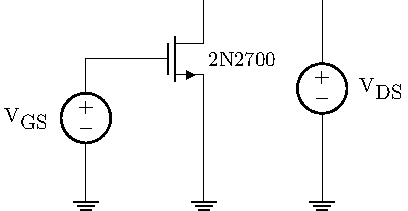
\includegraphics{circuits/circuit.pdf}
  \caption{Circuit for the Lab.}
  \label{fig:circuit}
\end{figure}

Finding $k_n$:

\[
  k_n = k_n'\Big( \frac{W}{L} \Big)
\]

\[
  V_{OV} = V_{GS} - V_t
\]

\[
  i_D = \frac{1}{2} k_n'\Big( \frac{W}{L} \Big) V_{OV}^2
\]

\[
  i_D = \frac{1}{2} k_n (V_{GS} - V_t)^2
\]

\begin{equation}
  k_n = \frac{2 i_D}{(V_{GS} - V_t)^2}
  \label{eq:kn}
\end{equation}

\section{Results}

\begin{figure}
  \centering
  \twosubfigures{../plots/pdf/sim_sweep_vgs.pdf}{Simulated}{fig:vgs_simulated}
                {../plots/pdf/sweep_vgs.pdf}{Measured}{fig:vgs_measured}
  \caption{Sweep V$_{GS}$}
  \label{fig:sweep_vgs}
\end{figure}

\begin{figure}
  \centering
  \twosubfigures{../plots/pdf/sim_sweep_vds.pdf}{Simulated}{fig:vds_simulated}
                {../plots/pdf/sweep_vds.pdf}{Measured}{fig:vds_measured}
  \caption{Sweep V$_{GS}$}
  \label{fig:sweep_vds}
\end{figure}


\section{Conclusion}

\end{document}
